\documentclass[12pt,a4paper]{report}

% Pacotes para acentuação e formatação
\usepackage[utf8]{inputenc}
\usepackage[T1]{fontenc}
\usepackage[brazil]{babel}
\usepackage{setspace}    % Para espaçamento
\usepackage{lipsum}      % Texto de exemplo (remova se não precisar)
\usepackage{graphicx}

\begin{document}
	
	% ----------- CAPA -----------
	\begin{titlepage}
		\centering
		\vspace*{5cm} % Espaço do topo
		
		{\Huge\bfseries Arquitetura de Computadores I\par} % Título
		
		\vspace{0.5cm}
		{\Large 2025/2\par} % Ano
		
		\vfill
		{\large Nicolas Ramos Carreira\par} % Nome
		
		\vspace*{2cm}
	\end{titlepage}
	
	% ----------- SUMÁRIO -----------
	\tableofcontents
	\newpage
	
	% ----------- CONTEÚDO -----------
	\chapter{Importância da matéria}
	Esta é sem dúvidas uma das disciplinas mais importantes para um Cientista da Computação, pois sem ela:
	
	\begin{itemize}
		\item Não saberemos como o computador funciona de fato
		\item Não seremos programadores tão bons como podemos ser
		\item Seremos mais sucessetiveis a cometer determinados erros
		
	\end{itemize}
	% Exemplo com texto fictício:
	%\lipsum[1]
	
	\chapter{O que aprenderemos}
	\section{Computadores são burros para fazer cálculos}
	\subsection{A conta: (43,1 - 43,2) + 1}
	\subsection{Propriedades matemáticas}
	\section{Como o Software roda no Hardware}
	
	\section{A memória}
	\subsection{O que é de fato?}
	Muitos programas dependem basicamente da memória RAM, mas a memória RAM não existe, é uma abstração limitada. O que existe é um complexo
	sistema hierárquico de memórias diferentes.
	
	Um exemplo disso é que temos a memória "Registradora", que se encontra no topo da hierarquia. Ela é a memória mais rápida que existe e que roda na mesma velocidade da CPU (ela fica dentro da CPU).
	
	Além disso, temos as memórias cach, que dão suporte a memória registradora.
	
	\begin{center}

		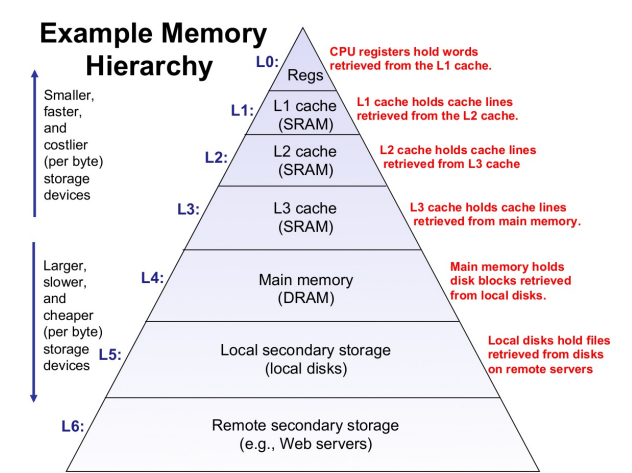
\includegraphics[width=8cm,height=5cm,keepaspectratio=false]{imagens-teoria/hierarquia_memoria.png}
		
	\end{center}
	
	\subsection{Bugs no referenciamento de memória são perniciosos}
	Quando estamos fazendo nosso programa, poderemos nos deparar com bugs de memória. Esses bugs podem ser bastante trabalhosos e chatos de lidar. Isso porque são bugs dificeis de serem debuggados
	\subsection{O porquê entender}
	Dado o contexto anterior, para ser um bom programador, você precisará entender a representação em nível de máquina, na memória, das estruturas de dados e como elas funcionam, pois isso faz uma grande diferença na sua habilidade de evitar e lidar com problemas de referenciamento de memória e vulnerabilidades no seu programa.
	
	Sendo assim, precisaremos entender:
	\begin{itemize}
		\item A hierarquia de memória
		\item Como a arquitetura da memória
		e linguagens como C podem levar a bugs de referenciamento de memória que são complicados de debugar e que podem ser distantes do tempo e espaço
		\item Que a performance da memória
		não é uniforme e que é necessário otimizar
		para o baixo nível também
	\end{itemize}  
	
	\section{Insight sobre abstrações}
	Boa parte do que sabemos sobre os computadores são, na verdade abstrações. No mais baixo nível possível, para o computador realizar uma soma, ele move eletrons.
	
	Sabendo disso, ao longo do tempo, nós fomos precisando de abstrações para representar isso. Foi então que vieram os componentes eletronicos. Porém nós ainda não conseguimos programar/interagir com isso. Dessa forma, abstrairam mais e criaram os circuitos elétricos analogicos. Ainda assim, não conseguimos programar/interagir bem com isso, então criaram a abstração dos circuitos digitais (0, 1, portas lógicas).
	
	\chapter{Introdução}
	\section{Acerca da história}
	
	\section{Discussão sobre performance}
	\section{Falando sobre software}
	\section{Arquitetura de von neumann}
	
	
\end{document}
